% Para facilitar a manutenção é sempre melhore criar um arquivo por capitulo, para exemplo isso não é necessário 

%---------------------------------------------------------------------------------------
\chapter{Escalabilidade}

O quesito ‘escalabilidade’ é muito abordado e de extrema importância atualmente, principalmente devido ao enorme fluxo de dados que corre dentre os sistemas e aplicações. A escalabilidade diz respeito a facilidade de crescimento da infraestrutura da aplicação de forma saudável, sem grandes impactos nos custos ferramentais e humanos e no desempenho da aplicação. Essa adaptabilidade pode estar relacionada com a implementação de novas funcionalidades, novas demandas de mercado, inserção em requisições legislativas e projetos de inovação, por exemplo. 

O projeto conta com ferramentas muito atuais, que já trazem consigo muito fortemente o conceito de escalabilidade, como o Heroku e o Docker, o primeiro que ganha cada vez mais espaço de mercado como uma Platform as a Service (PaaS), em que a solução permite que o desenvolvedor se desapegue de detalhes estruturais, trazendo maior facilidade de manutenção e maior agilidade de deploy, já o segundo possibilita a criação de ambientes virtuais completos, os chamados contêineres, que podem até mesmo ter seu crescimento automatizado de acordo com a demanda de requisições, gerando novos contêineres semelhantes, por exemplo. 

Por se tratar de um modelo de aplicação com pouca concorrência em mercado, existem chances relevantes de crescimento, assim, é possível que haja a necessidade de escalada da aplicação em um futuro breve, tendo isso em consideração, as ferramentas anteriormente citadas se encaixam muito bem nessa possível necessidade futura. 


%---------------------------------------------------------------------------------------
\chapter{Critérios de segurança}

\begin{itemize}
    \item A aplicação está de acordo com a Lei Geral de Proteção de Dados (LGPD, Lei nº13.709/2018). 
    
    \item Os dados que serão coletados e utilizados são: Como o usuário gostaria de ser chamado, foto do usuário opcional, data de nascimento, e-mail, neuroatipicidade da criança, localização aproximada opcional e senha. Não é obrigatório a publicação nem carregamento de dados pessoais que não queira disponibilizar ao público. 
    
    \item Para maior garantia de segurança, o armazenamento da senha será feito com criptografia e os dados dos usuários obterão total sigilo, sendo visíveis apenas pelo próprio usuário e por administradores do sistema em situações que sejam necessárias. 
    
    \item Os dados não sensíveis dos usuários (como nome de usuário e foto de perfil) serão visíveis para todos os usuários cadastrados, já dados sensíveis serão visualizáveis apenas pelo próprio usuário e, se necessário, pelos administradores da plataforma. 
    
    \item Os dados terão a sua integridade mantida, ou seja, não sofrerão alterações indevidas sem autorização do usuário, para que não possam vir a corromper a veracidade das informações. 
    
    \item Caso o usuário opte por encerrar sua conta, os seus dados pessoais não ficarão mais visíveis para outros usuários e seu perfil não deverá mais ser encontrado nas buscas dentro do aplicativo. Em 30 dias após o encerramento da conta todos os dados e informações da conta encerrada serão excluídos. 
\end{itemize}

%---------------------------------------------------------------------------------------
\chapter{Tecnologias a serem utilizadas}

Para o lado do cliente, iremos utilizar o React Native com Typescript junto a ferramenta Expo para testar o app com as APIs nativas do Android que essa ferramenta disponibiliza.

Já para o lado do servidor, utilizaremos Node.js com Typescript e framework NestJS para a construção da API, MongoDB como banco de dados, Prisma como ORM, Cloudinary como storage e para documentação de API, a especificação OpenAPI.

Para o ambiente de desenvolvimento, será utilizado o Docker a fim de obtermos facilidade em executar o projeto independente do Sistema Operacional local.

A hospedagem se dará por meio da Play Store para o app em React Native, do Heroku para o backend em Node.js e do MongoDB Atlas para o banco de dados.
Todo o versionamento será feito por meio das plataformas Github e Subversion.

Para realizar a prototipação das interfaces, será utilizada a ferramenta Figma e a construção de fluxos e brainstorms da equipe se darão por meio do Miro e Whimsical.

Por fim, para o gerenciamento do projeto, utilizaremos o Trello para registro de backlog e acompanhamento do status de desenvolvimento das histórias, o Discord para realização das cerimônias semanais da equipe e o WhatsApp para comunicações rápidas e mais urgentes entre o time.

\chapter{Manutenibilidade da aplicação desenvolvida}

\section{Ferramentas compatíveis com as tecnologias escolhidas para Testes automatizados e Análise Estática}
Usaremos Jest, um framework JavaScript para testes automatizados, e ESLint para análise estática do código.

\section{Sistemas de log para toda a aplicação}
Papertrail será o sistema de log que utilizaremos para mapear o comportamento da API em Node.js.

\section{Um processo de Integração Contínua}
A partir das Github Actions iremos estabelecer nosso workflow de CI (Continuous Integration).

\section{Especificação do “Coding Convention” (seja o próprio da linguagem, ou um criado/adaptado pela equipe)}
Usaremos o padrão recomendado pelo próprio ESLint para adequar:
\begin{itemize}
    \item Layout e formatação;
    \item Sugestão de alternativas para implementação do código (como, por exemplo, o uso do padrão camelCase para nomenclatura);
    \item Regras que visam corrigir possíveis problemas de lógica do código.
\end{itemize}
Todas as especificações a serem utilizadas estão disponíveis em: https://eslint.org/docs/rules/

\section{Design Patterns pertinentes à aplicação}
Utilizaremos os padrões Observer, Singleton e Injeção de Dependência.

\chapter{Diagrama de classes do sistema}
\begin{sidewaysfigure}[htb]

    \centering
	\caption{\label{fig_diag_virado}Diagrama de classes do sistema}
	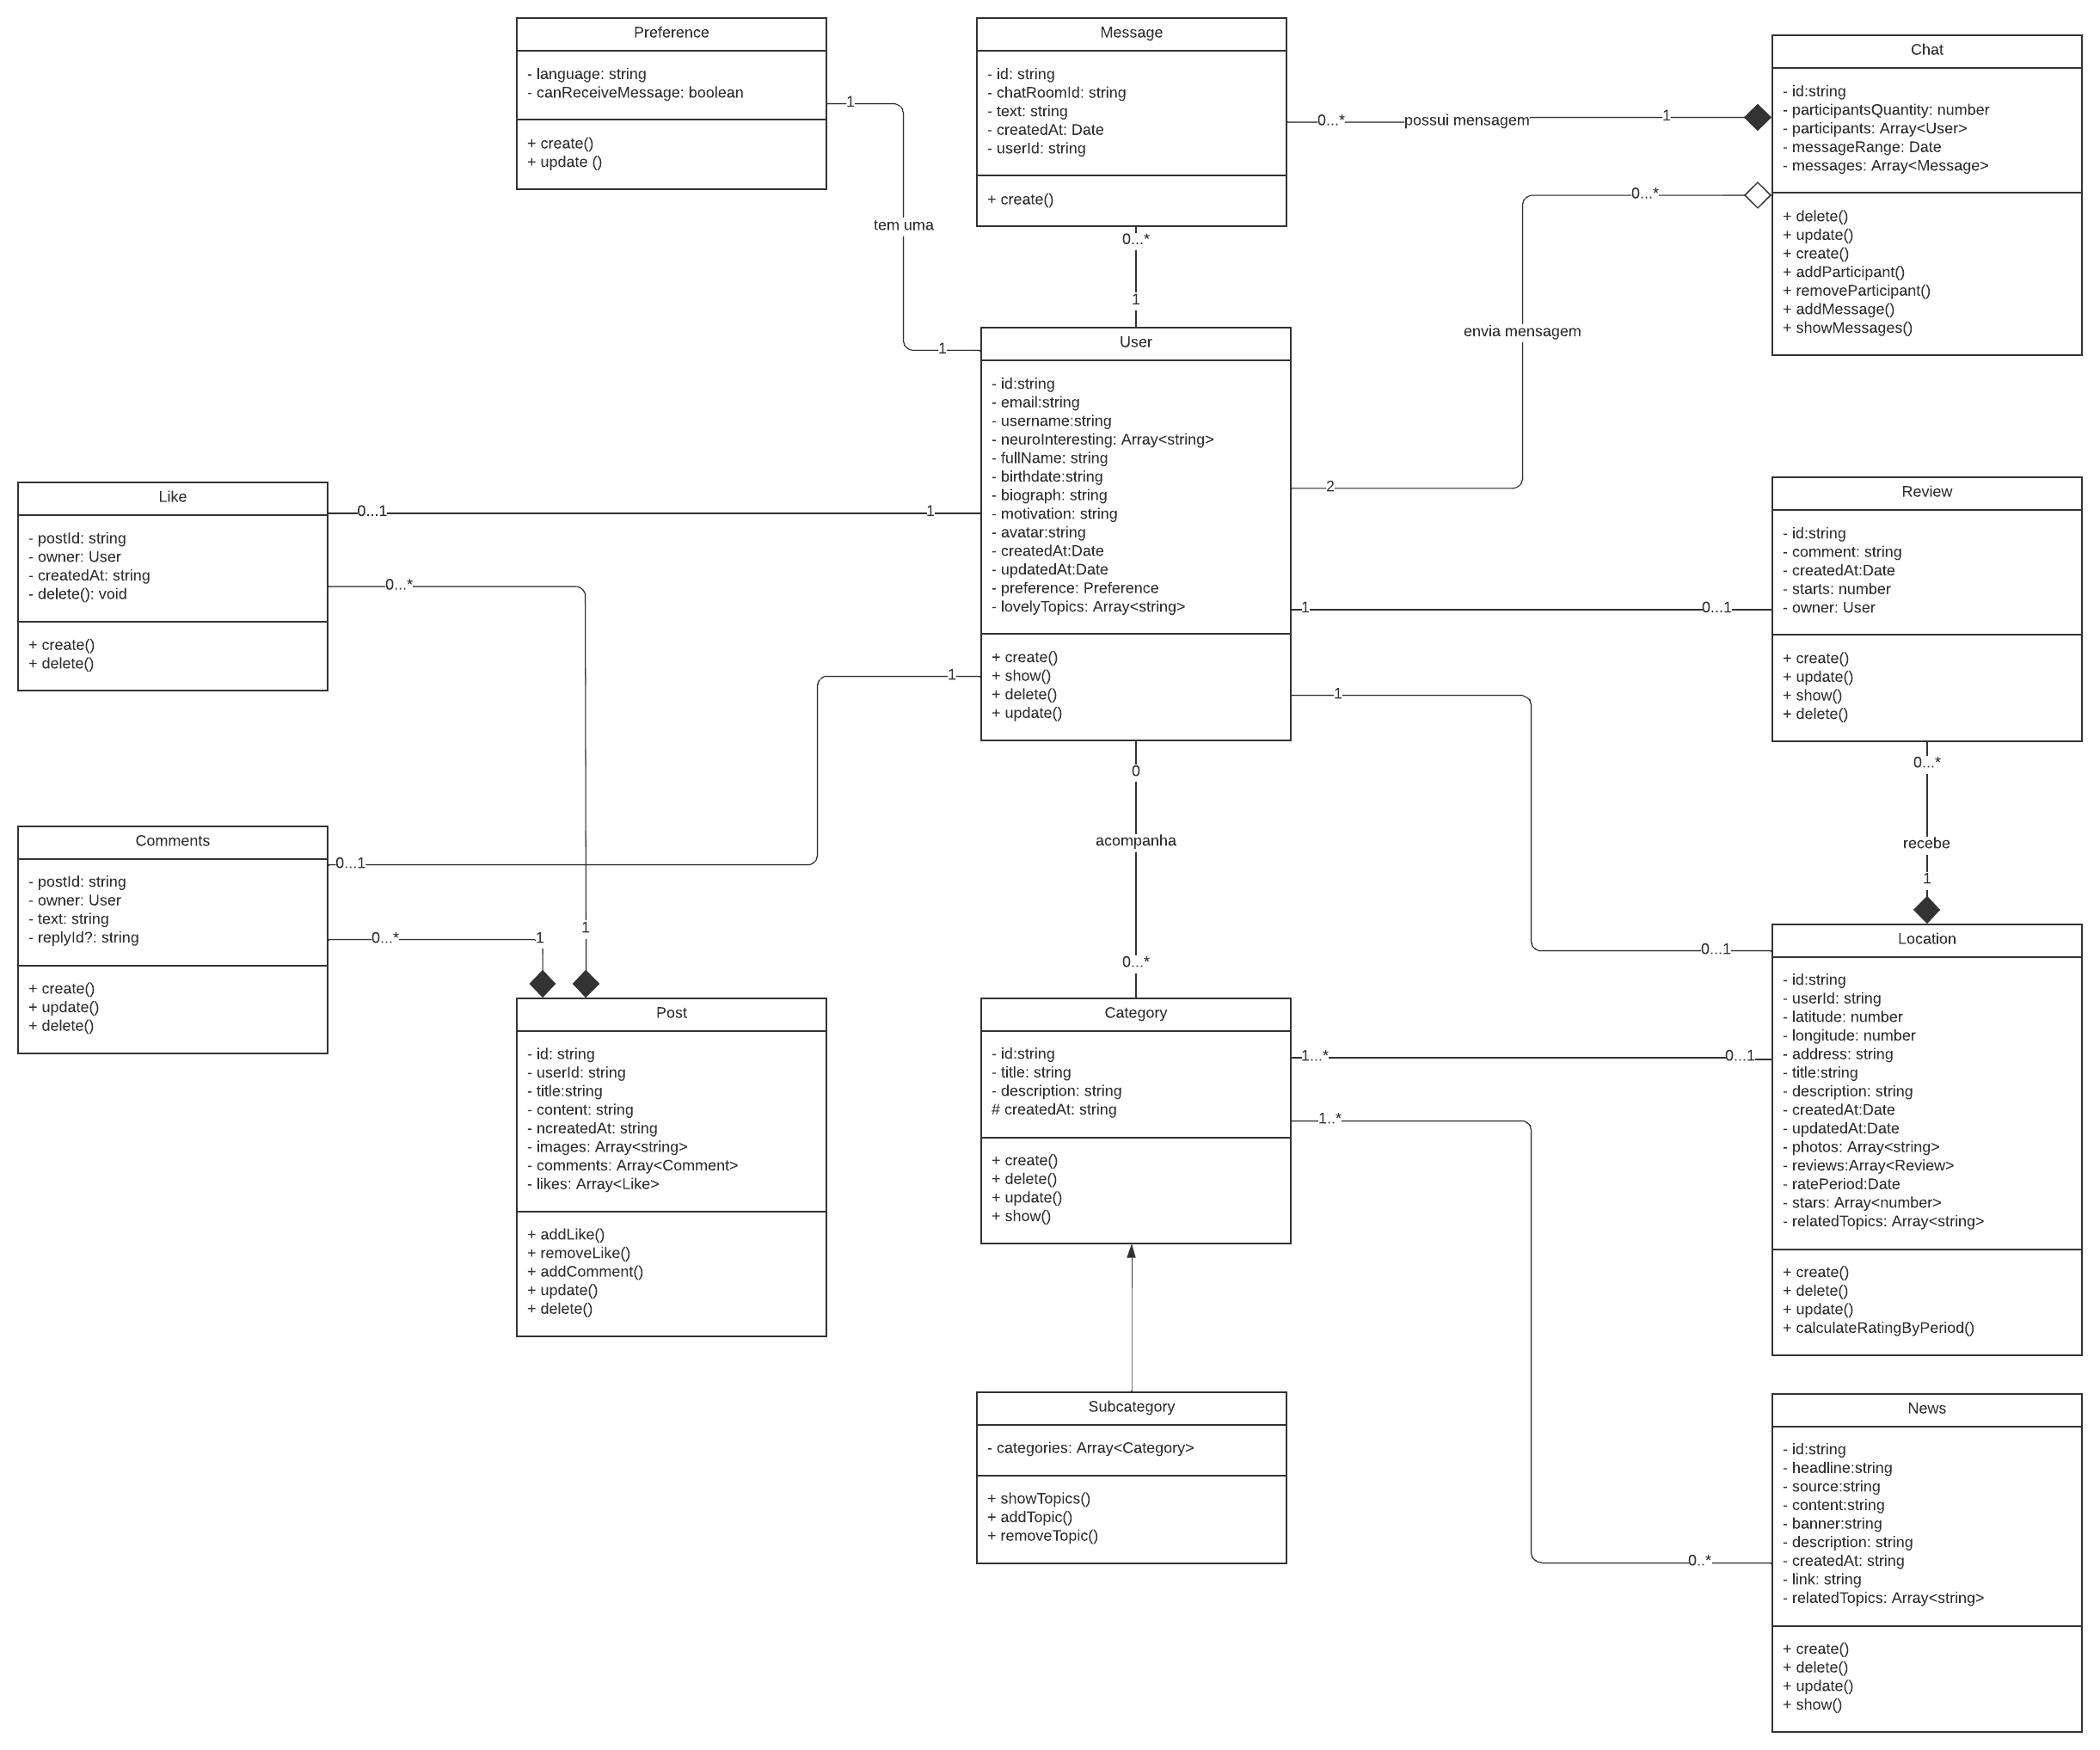
\includegraphics[width=0.9\textwidth]{anexos/diagrama.png}

	\end{sidewaysfigure}
%---------------------------------------------------------------------------------------




